\documentclass{beamer}
\usetheme{Madrid}
\usecolortheme{whale}

\usepackage[utf8]{inputenc}
\usepackage[T1]{fontenc}
\usepackage[french]{babel}
\usepackage{graphicx}
\usepackage{tikz}
\usepackage{booktabs}
\usepackage{listings}

% Configuration des chemins d'images
\graphicspath{{./01-preliminary/}}

% Configuration TikZ
\usetikzlibrary{calc}
\tikzset{
    gridstyle/.style={step=1cm, gray!40, very thin},
    borderstyle/.style={thick, black},
    bittext/.style={font=\tiny\sffamily},
    bitzero/.style={font=\tiny, gray!40},
    bitone/.style={font=\tiny\bfseries}
}

% --- INFO PRÉSENTATION ---
\title[Jeu des Amazones]{Implémentation du Jeu des Amazones}
\subtitle{Projet de Programmation - Master 1 Informatique}
\author{Équipe PDP}
\institute[Université de Bordeaux]{Université de Bordeaux}
\date{\today}

\begin{document}

% -----------------------------------------------------------------------------
%   SLIDE DE TITRE
% -----------------------------------------------------------------------------
\begin{frame}
    \titlepage
\end{frame}

% -----------------------------------------------------------------------------
%   SOMMAIRE
% -----------------------------------------------------------------------------
\begin{frame}{Plan de la présentation}
    \tableofcontents
\end{frame}

% -----------------------------------------------------------------------------
%   1. INTRODUCTION
% -----------------------------------------------------------------------------
\section{Présentation du Jeu}
\begin{frame}{Le Jeu des Amazones}
    \begin{columns}
        \begin{column}{0.5\textwidth}
            \textbf{Règles principales :}
            \begin{itemize}
                \item Plateau $10 \times 10$.
                \item 2 joueurs (Blanc vs Noir).
                \item 4 Amazones par joueur.
                \item \textbf{But :} Bloquer l'adversaire (dernier à jouer gagne).
            \end{itemize}
            
            \vspace{0.5cm}
            \textbf{Un tour de jeu :}
            \begin{enumerate}
                \item \textbf{Déplacement} (type Reine échecs).
                \item \textbf{Tir de flèche} (bloque une case).
            \end{enumerate}
        \end{column}
        \begin{column}{0.5\textwidth}
            \centering
            % Miniature du plateau (TikZ simplifié)
            \begin{tikzpicture}[scale=0.3]
                \draw[step=1cm, gray!40, very thin] (0,0) grid (10,10);
                \draw[thick] (0,0) rectangle (10,10);
                % Quelques amazones
                \fill[blue!60] (3,0) rectangle (4,1); \node[white, tiny] at (3.5,0.5) {W};
                \fill[red!60] (3,9) rectangle (4,10); \node[white, tiny] at (3.5,9.5) {B};
                % Quelques flèches
                \fill[gray!60] (4,4) rectangle (5,5);
                \fill[gray!60] (5,5) rectangle (6,6);
            \end{tikzpicture}
        \end{column}
    \end{columns}
\end{frame}

% -----------------------------------------------------------------------------
%   2. ARCHITECTURE
% -----------------------------------------------------------------------------
\section{Architecture Logicielle}
\begin{frame}{Architecture Globale}
    \textbf{Pattern MVC (Modèle-Vue-Contrôleur)}
    \begin{itemize}
        \item Séparation stricte des responsabilités.
        \item Indépendance du moteur de jeu et de l'interface graphique.
    \end{itemize}
    
    \vspace{0.5cm}
    \centering
    % Inclusion du diagramme de classes s'il existe
    \includegraphics[width=0.8\textwidth, height=0.55\textheight, keepaspectratio]{class_diagram.png}
\end{frame}

% -----------------------------------------------------------------------------
%   3. BITBOARDS (CŒUR TECHNIQUE)
% -----------------------------------------------------------------------------
\section{Module Bitboard (Cœur Technique)}

\begin{frame}{Pourquoi les Bitboards ?}
    \textbf{Problème :} Représenter un plateau $10 \times 10$ efficacement.
    \begin{itemize}
        \item Tableau 2D \texttt{int[10][10]} ? $\rightarrow$ Lourd en mémoire, itérations lentes.
    \end{itemize}
    
    \textbf{Solution :} Trois entiers de 100 bits.
    \begin{enumerate}
        \item \texttt{white\_amazons}
        \item \texttt{black\_amazons}
        \item \texttt{blocked} (flèches)
    \end{enumerate}
    
    \textbf{Avantages :}
    \begin{itemize}
        \item Opérations logiques ($\&, |, \oplus$) en temps constant $O(1)$.
        \item Copie d'état instantanée (très utile pour l'IA).
    \end{itemize}
\end{frame}

\begin{frame}{Visualisation des Bitboards}
    \centering
    \begin{tikzpicture}[scale=0.25]
        % White Amazons
        \begin{scope}
            \draw[step=1cm, gray!30] (0,0) grid (10,10);
            \draw[thick] (0,0) rectangle (10,10);
            \fill[blue!40] (3,0) rectangle (4,1);
            \node[below] at (5,-0.5) {\tiny \texttt{white\_amazons}};
        \end{scope}
        
        \node at (11, 5) {\Large $|$};
        
        % Blocked
        \begin{scope}[xshift=12cm]
            \draw[step=1cm, gray!30] (0,0) grid (10,10);
            \draw[thick] (0,0) rectangle (10,10);
            \fill[gray!60] (4,4) rectangle (5,5);
            \node[below] at (5,-0.5) {\tiny \texttt{blocked}};
        \end{scope}
        
        \node at (23, 5) {\Large $=$};
        
        % Occupied
        \begin{scope}[xshift=24cm]
            \draw[step=1cm, gray!30] (0,0) grid (10,10);
            \draw[thick] (0,0) rectangle (10,10);
            \fill[blue!40] (3,0) rectangle (4,1);
            \fill[gray!60] (4,4) rectangle (5,5);
            \node[below] at (5,-0.5) {\tiny \texttt{occupied}};
        \end{scope}
    \end{tikzpicture}
\end{frame}

\begin{frame}{Le Problème du "Wrapping" (Pac-Man)}
    \textbf{Danger de l'indexation 1D :}
    \begin{itemize}
        \item Index $y \times 10 + x$.
        \item Case finale ligne 0 (index 9) + 1 $\rightarrow$ Début ligne 1 (index 10).
    \end{itemize}

    \vspace{0.5cm}
    \centering
    \begin{tikzpicture}[scale=0.6]
        \draw[step=1cm, gray!30] (0,0) grid (10,2);
        \draw[thick] (0,0) rectangle (10,2);
        
        \node at (9.5, 0.5) {9};
        \node at (0.5, 1.5) {10};
        
        % Flèche Pac-Man
        \draw[->, red, thick, dashed] (9.5, 0.5) -- (10.5, 0.5) 
            to[out=0, in=180] (-0.5, 1.5) -- (0.2, 1.5);
            
        \node[red, font=\small] at (5, 2.5) {Téléportation illégale !};
    \end{tikzpicture}
    
    \vspace{0.5cm}
    \textbf{Solution :} Masques de colonnes (\texttt{MASK\_COL\_J}) pour bloquer les débordements horizontaux.
\end{frame}

\begin{frame}{Validation et Déplacement}
    \textbf{1. Validation par Masques (AND) :}
    \begin{itemize}
        \item On crée un masque du chemin théorique.
        \item \texttt{if (chemin \& obstacles) != 0} $\rightarrow$ Collision.
    \end{itemize}
    
    \vspace{0.5cm}
    
    \textbf{2. Déplacement atomique (XOR + OR) :}
    \begin{enumerate}
        \item \textbf{XOR} : Libérer la case départ `from` (essentiel avant de tirer !).
        \item \textbf{OR} : Occuper la case arrivée `to`.
        \item \textbf{OR} : Placer la flèche `arrow`.
    \end{enumerate}
    
    \begin{center}
        \textcolor{blue}{\textbf{XOR}} $\rightarrow$ \textcolor{green}{\textbf{OR}} $\rightarrow$ \textcolor{gray}{\textbf{OR}}
    \end{center}
\end{frame}

% -----------------------------------------------------------------------------
%   4. RESEAU ET IA
% -----------------------------------------------------------------------------
\section{Réseau et IA}
\begin{frame}{Architecture Réseau}
    \begin{itemize}
        \item \textbf{Protocole UDP} : Découverte des parties (Broadcast).
        \item \textbf{Protocole TCP} : Échange des coups (Fiabilité).
    \end{itemize}
    \vspace{0.3cm}
    \centering
    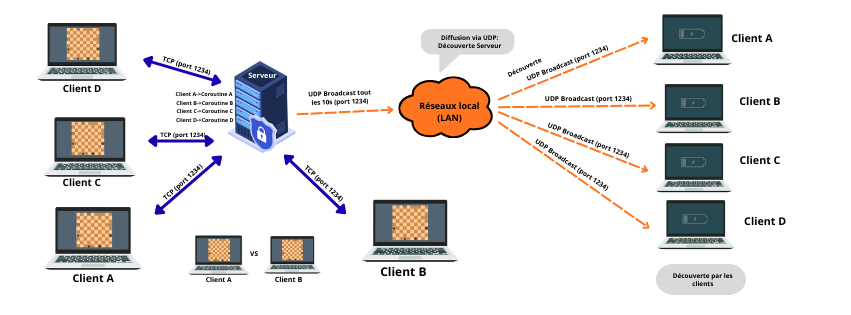
\includegraphics[width=0.7\textwidth, height=0.4\textheight, keepaspectratio]{shema_reseaux.png}
\end{frame}

% -----------------------------------------------------------------------------
%   5. CONCLUSION
% -----------------------------------------------------------------------------
\section{Conclusion}
\begin{frame}{Bilan du Projet}
    \textbf{Réalisations :}
    \begin{itemize}
        \item Moteur de jeu robuste et optimisé (Bitboards).
        \item Architecture MVC respectée.
        \item Interface graphique et mode réseau fonctionnels.
    \end{itemize}
    
    \vspace{0.5cm}
    \textbf{Améliorations futures :}
    \begin{itemize}
        \item Optimisation de l'IA (Monte Carlo Tree Search).
        \item Historique des coups et "Replay".
    \end{itemize}
    
    \vspace{1cm}
    \centering
    \Large \textbf{Merci de votre attention.} \\
    \small Avez-vous des questions ?
\end{frame}

\end{document}
